\documentclass[tikz,border=10pt]{standalone}
\usetikzlibrary{arrows.meta, calc, shapes.geometric, shadows}

\begin{document}
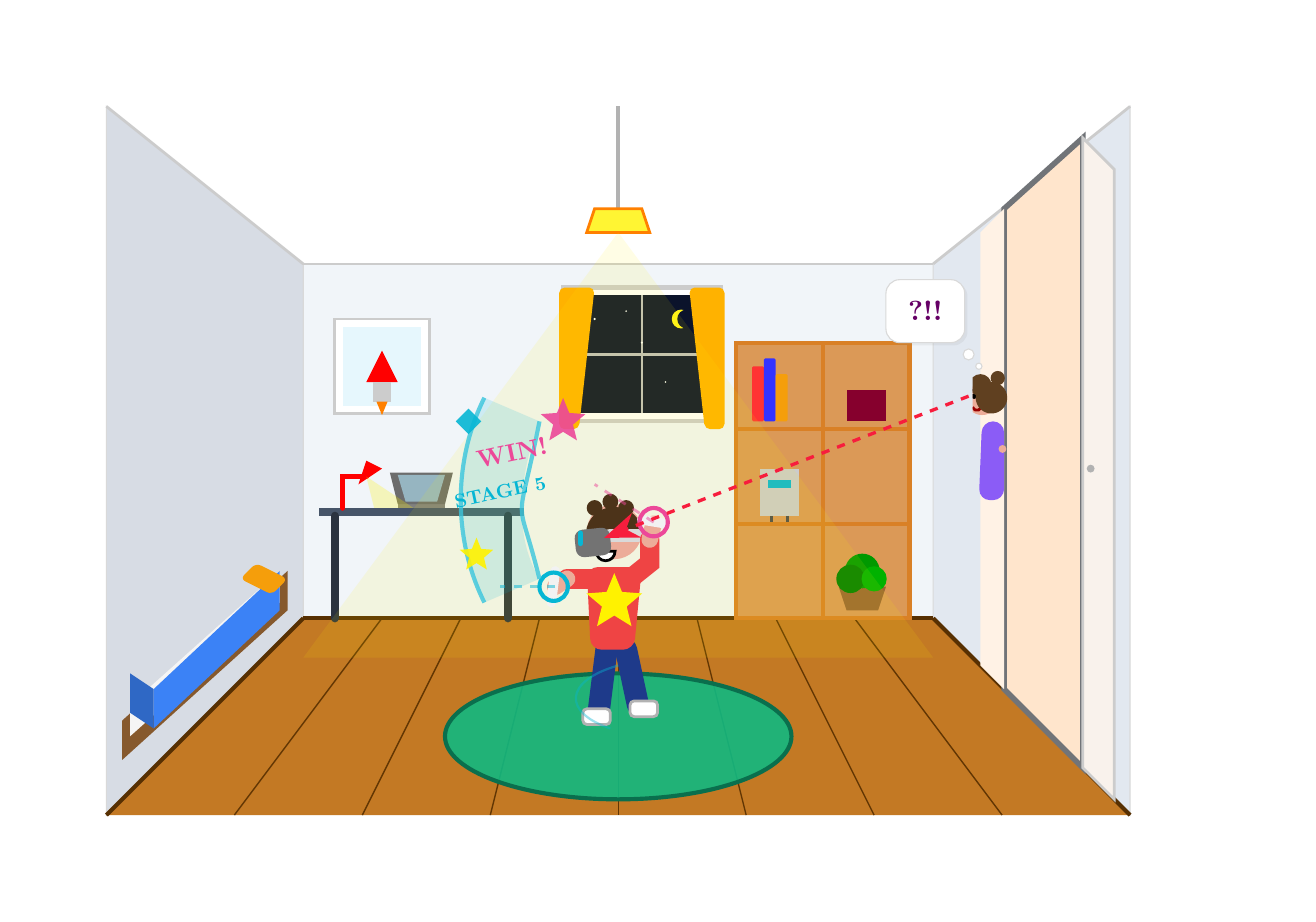
\begin{tikzpicture}
  % Colors
  \definecolor{sky}{HTML}{0B132B}      % Deep night sky
  \definecolor{wall}{HTML}{F1F5F9}     % Very light gray/blue wall
  \definecolor{sidewall}{HTML}{E2E8F0} % Slightly darker side wall
  \definecolor{floor}{HTML}{D97706}    % Warm woodfloor base
  \definecolor{rug}{HTML}{10B981}      % Emerald green rug
  \definecolor{desk}{HTML}{475569}     % Slate gray desk
  \definecolor{bed}{HTML}{3B82F6}      % Vibrant blue bedsheets
  \definecolor{pillow}{HTML}{F59E0B}   % Orange/yellow pillow
  \definecolor{neoncyan}{HTML}{06B6D4} % VR cyan glow
  \definecolor{neonpink}{HTML}{EC4899} % VR pink/magenta glow
  \definecolor{boytshirt}{HTML}{EF4444}% Dynamic red t-shirt
  \definecolor{boypants}{HTML}{1E3A8A} % Navy blue pants
  \definecolor{motherdress}{HTML}{8B5CF6} % Purple mother dress

  % Canvas bounding box for beautiful 4:3 aspect ratio
  \useasboundingbox (-8, -5.5) rectangle (8, 5.5);
  \fill[white] (-8, -5.5) rectangle (8, 5.5);

  % ==================== ROOM WALLS & FLOOR ====================
  % Coordinates of room corners
  % TL = Top Left, TR = Top Right, BR = Bottom Right, BL = Bottom Left
  % F = Front (closer to viewer)
  \coordinate (TL) at (-4.5, 2.5);
  \coordinate (TR) at (3.5, 2.5);
  \coordinate (BR) at (3.5, -2.0);
  \coordinate (BL) at (-4.5, -2.0);

  \coordinate (FTL) at (-7.0, 4.5);
  \coordinate (FTR) at (6.0, 4.5);
  \coordinate (FBR) at (6.0, -4.5);
  \coordinate (FBL) at (-7.0, -4.5);

  % Back Wall
  \fill[wall] (BL) rectangle (TR);
  \draw[gray!30, thin] (BL) rectangle (TR);

  % Left Wall
  \fill[sidewall!95!black] (FTL) -- (TL) -- (BL) -- (FBL) -- cycle;
  \draw[gray!30, thin] (FTL) -- (TL) -- (BL) -- (FBL) -- cycle;

  % Right Wall
  \fill[sidewall] (TR) -- (FTR) -- (FBR) -- (BR) -- cycle;
  \draw[gray!30, thin] (TR) -- (FTR) -- (FBR) -- (BR) -- cycle;

  % Floor
  \fill[floor!75!gray] (BL) -- (BR) -- (FBR) -- (FBL) -- cycle;

  % Floor Wood Planks (converging perspective lines)
  \foreach \i in {0,1,...,8} {
    \pgfmathsetmacro{\xback}{-4.5 + \i * 1.0}
    \pgfmathsetmacro{\xfront}{-7.0 + \i * 1.625}
    \draw[floor!45!black, line width=0.5pt] (\xback, -2.0) -- (\xfront, -4.5);
  }
  
  % Baseboards
  \draw[floor!40!black, line width=1.5pt] (BL) -- (BR);
  \draw[floor!40!black, line width=1.5pt] (BL) -- (FBL);
  \draw[floor!40!black, line width=1.5pt] (BR) -- (FBR);

  % Ceiling joint lines
  \draw[gray!40, line width=1pt] (TL) -- (TR);
  \draw[gray!40, line width=1pt] (TL) -- (FTL);
  \draw[gray!40, line width=1pt] (TR) -- (FTR);

  % ==================== WINDOW (Back Wall) ====================
  \fill[white, draw=gray!40, line width=1.5pt] (-1.2, 0.5) rectangle (0.8, 2.2);
  \fill[sky] (-1.1, 0.6) rectangle (0.7, 2.1);
  % Window grids
  \draw[gray!50, line width=0.8pt] (-0.2, 0.6) -- (-0.2, 2.1);
  \draw[gray!50, line width=0.8pt] (-1.1, 1.35) -- (0.7, 1.35);
  % Moon & Stars in the window
  \begin{scope}
    \clip (-1.1, 0.6) rectangle (0.7, 2.1);
    \fill[yellow!90] (0.3, 1.8) circle (0.12);
    \fill[sky] (0.37, 1.8) circle (0.12); % Crescent shadow
    \fill[white] (-0.8, 1.8) circle (0.015);
    \fill[white] (-0.4, 1.9) circle (0.012);
    \fill[white] (-0.2, 1.5) circle (0.015);
    \fill[white] (0.1, 1.0) circle (0.012);
  \end{scope}
  % Yellow Curtains
  \fill[orange!60!yellow, rounded corners=2pt] (-1.25, 0.4) -- (-1.0, 0.4) -- (-0.8, 2.2) -- (-1.25, 2.2) -- cycle;
  \fill[orange!60!yellow, rounded corners=2pt] (0.85, 0.4) -- (0.6, 0.4) -- (0.4, 2.2) -- (0.85, 2.2) -- cycle;

  % ==================== FURNITURE ====================
  % Poster on Back Wall
  \fill[white, draw=gray!40, line width=1pt] (-4.1, 0.6) rectangle (-2.9, 1.8);
  \fill[cyan!10] (-4.0, 0.7) rectangle (-3.0, 1.7);
  \fill[red] (-3.5, 1.4) -- (-3.7, 1.0) -- (-3.3, 1.0) -- cycle; % Rocket nose
  \fill[gray!40] (-3.62, 1.0) rectangle (-3.38, 0.75);           % Rocket body
  \fill[orange] (-3.57, 0.75) -- (-3.5, 0.58) -- (-3.43, 0.75) -- cycle; % Fire

  % Bed (Left side, against left wall)
  % Bed Base
  \fill[brown!70!black] (-6.8, -3.8) -- (-4.7, -1.9) -- (-4.7, -1.4) -- (-6.8, -3.3) -- cycle;
  % Mattress
  \fill[white!92!gray] (-6.7, -3.5) -- (-4.8, -1.8) -- (-4.8, -1.4) -- (-6.7, -3.1) -- cycle;
  % Bed Blanket (navy/blue)
  \fill[bed] (-6.4, -3.4) -- (-4.8, -1.9) -- (-4.8, -1.4) -- (-6.4, -2.9) -- cycle;
  \fill[bed!80!black] (-6.7, -3.2) -- (-6.4, -3.4) -- (-6.4, -2.9) -- (-6.7, -2.7) -- cycle;
  % Yellow Pillow
  \fill[pillow, rounded corners=2pt] (-4.9, -1.7) -- (-5.3, -1.5) -- (-5.1, -1.3) -- (-4.7, -1.5) -- cycle;

  % Desk (Back Wall, Left Side)
  \fill[desk] (-4.3, -0.7) rectangle (-1.7, -0.6);
  \draw[desk!60!black, line width=3pt, line cap=round] (-4.1, -0.7) -- (-4.1, -2.0);
  \draw[desk!60!black, line width=3pt, line cap=round] (-1.9, -0.7) -- (-1.9, -2.0);
  % Laptop on Desk
  \fill[gray] (-3.3, -0.6) rectangle (-2.7, -0.55);
  \fill[gray!85!black] (-3.3, -0.55) -- (-2.7, -0.55) -- (-2.6, -0.15) -- (-3.4, -0.15) -- cycle;
  \fill[cyan!30, opacity=0.6] (-3.2, -0.52) -- (-2.8, -0.52) -- (-2.7, -0.18) -- (-3.3, -0.18) -- cycle;
  % Red Desk Lamp
  \draw[red, line width=2pt, line cap=round] (-4.0, -0.6) -- (-4.0, -0.2) -- (-3.7, -0.2);
  \fill[red] (-3.8, -0.3) -- (-3.5, -0.1) -- (-3.7, 0.0) -- cycle;
  \fill[yellow, opacity=0.25] (-3.7, -0.2) -- (-3.1, -0.6) -- (-3.6, -0.6) -- cycle;

  % Bookshelf / Toy Shelf (Back Wall, Right Side)
  \fill[orange!30!brown!80] (1.0, -2.0) rectangle (3.2, 1.5);
  \draw[orange!40!brown, line width=1.5pt] (1.0, -2.0) rectangle (3.2, 1.5);
  % Dividers
  \draw[orange!40!brown, line width=1.5pt] (1.0, -0.8) -- (3.2, -0.8);
  \draw[orange!40!brown, line width=1.5pt] (1.0, 0.4) -- (3.2, 0.4);
  \draw[orange!40!brown, line width=1.5pt] (2.1, -2.0) -- (2.1, 1.5);
  % Shelf Contents
  % Books
  \fill[red!80, rounded corners=0.5pt] (1.2, 0.5) rectangle (1.35, 1.2);
  \fill[blue!80, rounded corners=0.5pt] (1.35, 0.5) rectangle (1.5, 1.3);
  \fill[pillow, rounded corners=0.5pt] (1.5, 0.5) rectangle (1.65, 1.1);
  \fill[purple!70!black] (2.4, 0.5) rectangle (2.9, 0.9);
  % Toy Robot
  \fill[gray!40] (1.3, -0.7) rectangle (1.8, -0.1);
  \fill[neoncyan] (1.4, -0.35) rectangle (1.7, -0.25);
  \draw[gray!60!black, line width=1pt] (1.45, -0.7) -- (1.45, -0.78);
  \draw[gray!60!black, line width=1pt] (1.65, -0.7) -- (1.65, -0.78);
  % Plant
  \fill[brown!80!black] (2.4, -1.9) -- (2.8, -1.9) -- (2.9, -1.6) -- (2.3, -1.6) -- cycle;
  \fill[green!60!black] (2.6, -1.4) circle (0.22);
  \fill[green!50!black] (2.45, -1.5) circle (0.18);
  \fill[green!70!black] (2.75, -1.5) circle (0.16);

  % Ceiling Lamp
  \draw[gray!60, line width=1.5pt] (-0.5, 4.5) -- (-0.5, 3.2);
  \fill[yellow!80, draw=orange, line width=1pt] (-0.8, 3.2) -- (-0.2, 3.2) -- (-0.1, 2.9) -- (-0.9, 2.9) -- cycle;
  \fill[yellow, opacity=0.1] (-0.5, 2.9) -- (-4.5, -2.5) -- (3.5, -2.5) -- cycle;

  % Emerald Green Rug on Floor
  \fill[rug, opacity=0.9] (-0.5, -3.5) ellipse (2.2 and 0.8);
  \draw[rug!60!black, line width=1.5pt] (-0.5, -3.5) ellipse (2.2 and 0.8);

  % ==================== THE BOY (VR Player) ====================
  % Left Leg (standing dynamically)
  \draw[boypants, line width=8pt, line cap=round] (-0.75, -3.2) -- (-0.65, -2.4);
  % Right Leg (slightly bent back)
  \draw[boypants, line width=8pt, line cap=round] (-0.25, -3.1) -- (-0.4, -2.4);
  % Shoes
  \fill[white, draw=gray!60, line width=1pt, rounded corners=1.5pt] (-0.95, -3.35) rectangle (-0.6, -3.15);
  \fill[white, draw=gray!60, line width=1pt, rounded corners=1.5pt] (-0.35, -3.25) rectangle (0.0, -3.05);

  % Torso (leaning left/forward, dynamic)
  \fill[boytshirt, rounded corners=4pt] (-0.85, -2.4) -- (-0.3, -2.4) -- (-0.2, -1.35) -- (-0.9, -1.35) -- cycle;
  % Shirt Logo (Yellow star)
  \node[star, star points=5, star point ratio=2.25, fill=yellow, minimum size=0.25cm] at (-0.55, -1.8) {};

  % Head & Face
  \fill[pink!70!brown] (-0.55, -0.9) circle (0.35); % skin
  \draw[black, fill=white, line width=1pt] (-0.78, -1.15) arc (180:360:0.12) -- cycle; % happy open mouth smile

  % Hair
  \fill[brown!40!black] (-0.9, -0.85) .. controls (-0.8, -0.5) and (-0.3, -0.5) .. (-0.2, -0.85) -- (-0.2, -0.95) .. controls (-0.4, -0.9) and (-0.7, -0.9) .. (-0.9, -0.95) -- cycle;
  \fill[brown!40!black] (-0.8, -0.6) circle (0.1);
  \fill[brown!40!black] (-0.6, -0.52) circle (0.1);
  \fill[brown!40!black] (-0.4, -0.6) circle (0.1);

  % VR Headset
  % Headset Strap
  \draw[gray!30, line width=5pt, line cap=round] (-0.6, -0.95) -- (-0.25, -0.95);
  % Main Headset Box (facing left/front)
  \fill[gray!90!black, rounded corners=3pt, rotate around={6:(-0.7, -1.0)}] (-1.05, -1.2) rectangle (-0.6, -0.85);
  % Cyan LED Glow on VR
  \draw[neoncyan, line width=2pt, line cap=round] (-0.98, -1.05) -- (-0.98, -0.92);

  % Arms & Controllers
  % Left Arm (extending forward/left)
  \draw[boytshirt, line width=7pt, line cap=round] (-0.75, -1.5) -- (-1.15, -1.5);
  \draw[pink!70!brown, line width=6pt, line cap=round] (-1.15, -1.5) -- (-1.3, -1.6);
  % Controller 1 (white + cyan glow)
  \draw[white!90!gray, line width=3.5pt, line cap=round] (-1.3, -1.4) -- (-1.35, -1.8);
  \draw[neoncyan, line width=1.5pt] (-1.32, -1.6) circle (0.18);
  
  % Right Arm (extending upwards/right)
  \draw[boytshirt, line width=7pt, line cap=round] (-0.35, -1.5) -- (-0.1, -1.3) -- (-0.1, -1.0);
  \draw[pink!70!brown, line width=6pt, line cap=round] (-0.1, -1.0) -- (-0.05, -0.8);
  % Controller 2 (white + pink glow)
  \draw[white!90!gray, line width=3.5pt, line cap=round] (-0.2, -0.75) -- (0.1, -0.8);
  \draw[neonpink, line width=1.5pt] (-0.05, -0.78) circle (0.18);

  % ==================== VR WORLD HOLOGRAM EFFECTS ====================
  % Semi-translucent glowing virtual screen in front of boy
  \fill[neoncyan, opacity=0.15] (-2.2, -1.8) .. controls (-2.6, -1.0) and (-2.6, 0.0) .. (-2.2, 0.8) 
                            -- (-1.5, 0.5) .. controls (-1.8, -0.3) and (-1.8, -1.0) .. (-1.5, -1.5) -- cycle;
  \draw[neoncyan!80, line width=1.5pt, opacity=0.8] (-2.2, -1.8) .. controls (-2.6, -1.0) and (-2.6, 0.0) .. (-2.2, 0.8);
  \draw[neoncyan!80, line width=1.5pt, opacity=0.8] (-1.5, -1.5) .. controls (-1.8, -0.3) and (-1.8, -1.0) .. (-1.5, 0.5);
  
  % Game UI texts
  \node[rotate=12, scale=0.7, neoncyan] at (-2.0, -0.4) {\bf STAGE 5};
  \node[rotate=12, scale=0.9, neonpink] at (-1.85, 0.1) {\bf WIN!};
  
  % Floating glowing objects
  \node[star, star points=5, star point ratio=2.25, fill=neonpink, minimum size=0.25cm, scale=0.8, opacity=0.9] at (-1.2, 0.5) {};
  \node[star, star points=5, star point ratio=2.25, fill=yellow, minimum size=0.25cm, scale=0.6, opacity=0.9] at (-2.3, -1.2) {};
  \node[diamond, fill=neoncyan, minimum size=0.2cm, scale=0.7, opacity=0.9] at (-2.4, 0.5) {};
  
  % Cybernetic motion / action lines around boy
  \draw[neoncyan, opacity=0.5, dashed, line width=1pt] (-1.3, -1.6) -- (-2.0, -1.6);
  \draw[neonpink, opacity=0.5, dashed, line width=1pt] (-0.05, -0.78) -- (-0.8, -0.3);
  \draw[neoncyan, opacity=0.4, line width=0.8pt] (-0.5, -2.6) .. controls (-1.2, -2.8) and (-1.2, -3.2) .. (-0.6, -3.4);

  % ==================== THE MOTHER & DOORWAY ====================
  % Right Wall Doorway (bright hallway light casting in)
  \fill[orange!20, draw=sidewall!50!black, line width=2pt] (4.4, -2.9) -- (5.4, -3.9) -- (5.4, 4.1) -- (4.4, 3.2) -- cycle;
  
  % Swing Open Door panel
  \fill[white!90!brown, draw=gray!40, line width=1pt] (5.4, -3.9) -- (5.8, -4.3) -- (5.8, 3.7) -- (5.4, 4.1) -- cycle;
  \fill[gray!60] (5.5, -0.1) circle (0.05); % Door handle

  % Hallway wall showing through door frame
  \fill[orange!10] (4.4, -2.9) -- (4.4, 3.2) -- (4.1, 2.9) -- (4.1, -2.6) -- cycle;

  % The Mother (peeking around the door frame)
  \begin{scope}
    % Clip her body behind the room's main wall to make her look like she's peeking out
    \clip (4.0, -3.5) rectangle (5.4, 3.5);
    
    % Mother Dress / Body
    \fill[motherdress, rounded corners=4pt] (4.4, 0.5) -- (4.12, 0.5) -- (4.08, -0.5) -- (4.4, -0.5) -- cycle;
    
    % Mother Face
    \fill[pink!70!brown] (4.12, 0.78) circle (0.2);
    % Peeking Nose
    \draw[pink!60!brown!80!black, line width=1.5pt] (3.97, 0.78) -- (3.92, 0.78);
    % Curious Eye looking left
    \fill[black] (4.02, 0.82) circle (0.035);
    % Surprised/raised eyebrow
    \draw[black!80, line width=0.8pt] (3.98, 0.89) arc (120:60:0.08);
    % Friendly gentle smile
    \draw[red!60!black, line width=1pt] (4.0, 0.68) arc (200:340:0.06);

    % Hair & Hair Bun
    \fill[brown!50!black] (4.1, 0.96) circle (0.14);
    \fill[brown!50!black] (4.24, 0.8) circle (0.2);
    \fill[brown!50!black] (4.32, 1.05) circle (0.09); % Hair bun

    % Hand holding the door frame
    \fill[pink!70!brown] (4.38, 0.15) circle (0.05);
  \end{scope}

  % ==================== SIGHTLINE & EXPRESSIONS ====================
  % Dotted sightline from Mother's eye to VR Headset
  \draw[red!60!neonpink, dashed, line width=1.2pt, -{Stealth[scale=1.5]}] (3.95, 0.82) -- (-0.68, -0.98);
  
  % Mother's Cute Surprise thought bubble
  \begin{scope}[shift={(3.4, 1.9)}]
    % Bubble backdrop with dropshadow
    \fill[white, draw=gray!30, rounded corners=5pt, drop shadow={opacity=0.1, shadow xshift=1pt, shadow yshift=-1pt}] (-0.5, -0.4) rectangle (0.5, 0.4);
    \node at (0, 0) {\bf\color{violet!80!black}?!!};
    % Small tail bubbles
    \fill[white, draw=gray!30] (0.55, -0.55) circle (0.07);
    \fill[white, draw=gray!30] (0.68, -0.7) circle (0.04);
  \end{scope}

\end{tikzpicture}
\end{document}
